\chapter{Pick and place points}

\section{Bumpiness}
\begin{equation}\label{bumpiness}
B = \sum_{i=1}^{n} | \textrm{path}(i)- \textrm{path}(i-1) | 
\end{equation}

Where $n$ is the number of points composing the path. The path with the lowest bumpiness value, which corresponds to the path with the less and smallest height changes, is selected as the unfold direction, Fig. \ref{candidate_paths}.



\begin{figure}[thpb]
    \centering
    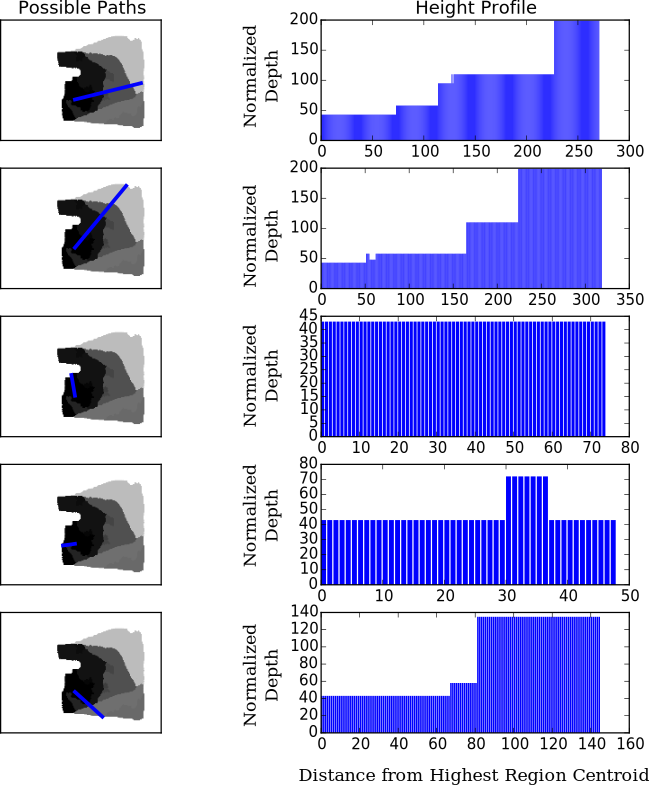
\includegraphics[width=0.48\textwidth]{figures/candidate_paths.pdf}
    \caption{On the left side, the candidate paths are shown. On the right side, the height profile of each path is shown. Notice that the depth sensor computes the distance to the object from itself, so that a low value in the bar plot means a closer object to the sensor, so it is a region with more height with respect to the table.}
    \label{candidate_paths}
\end{figure}

\section{Pick and place points}
\begin{figure}[thpb]
    \centering
    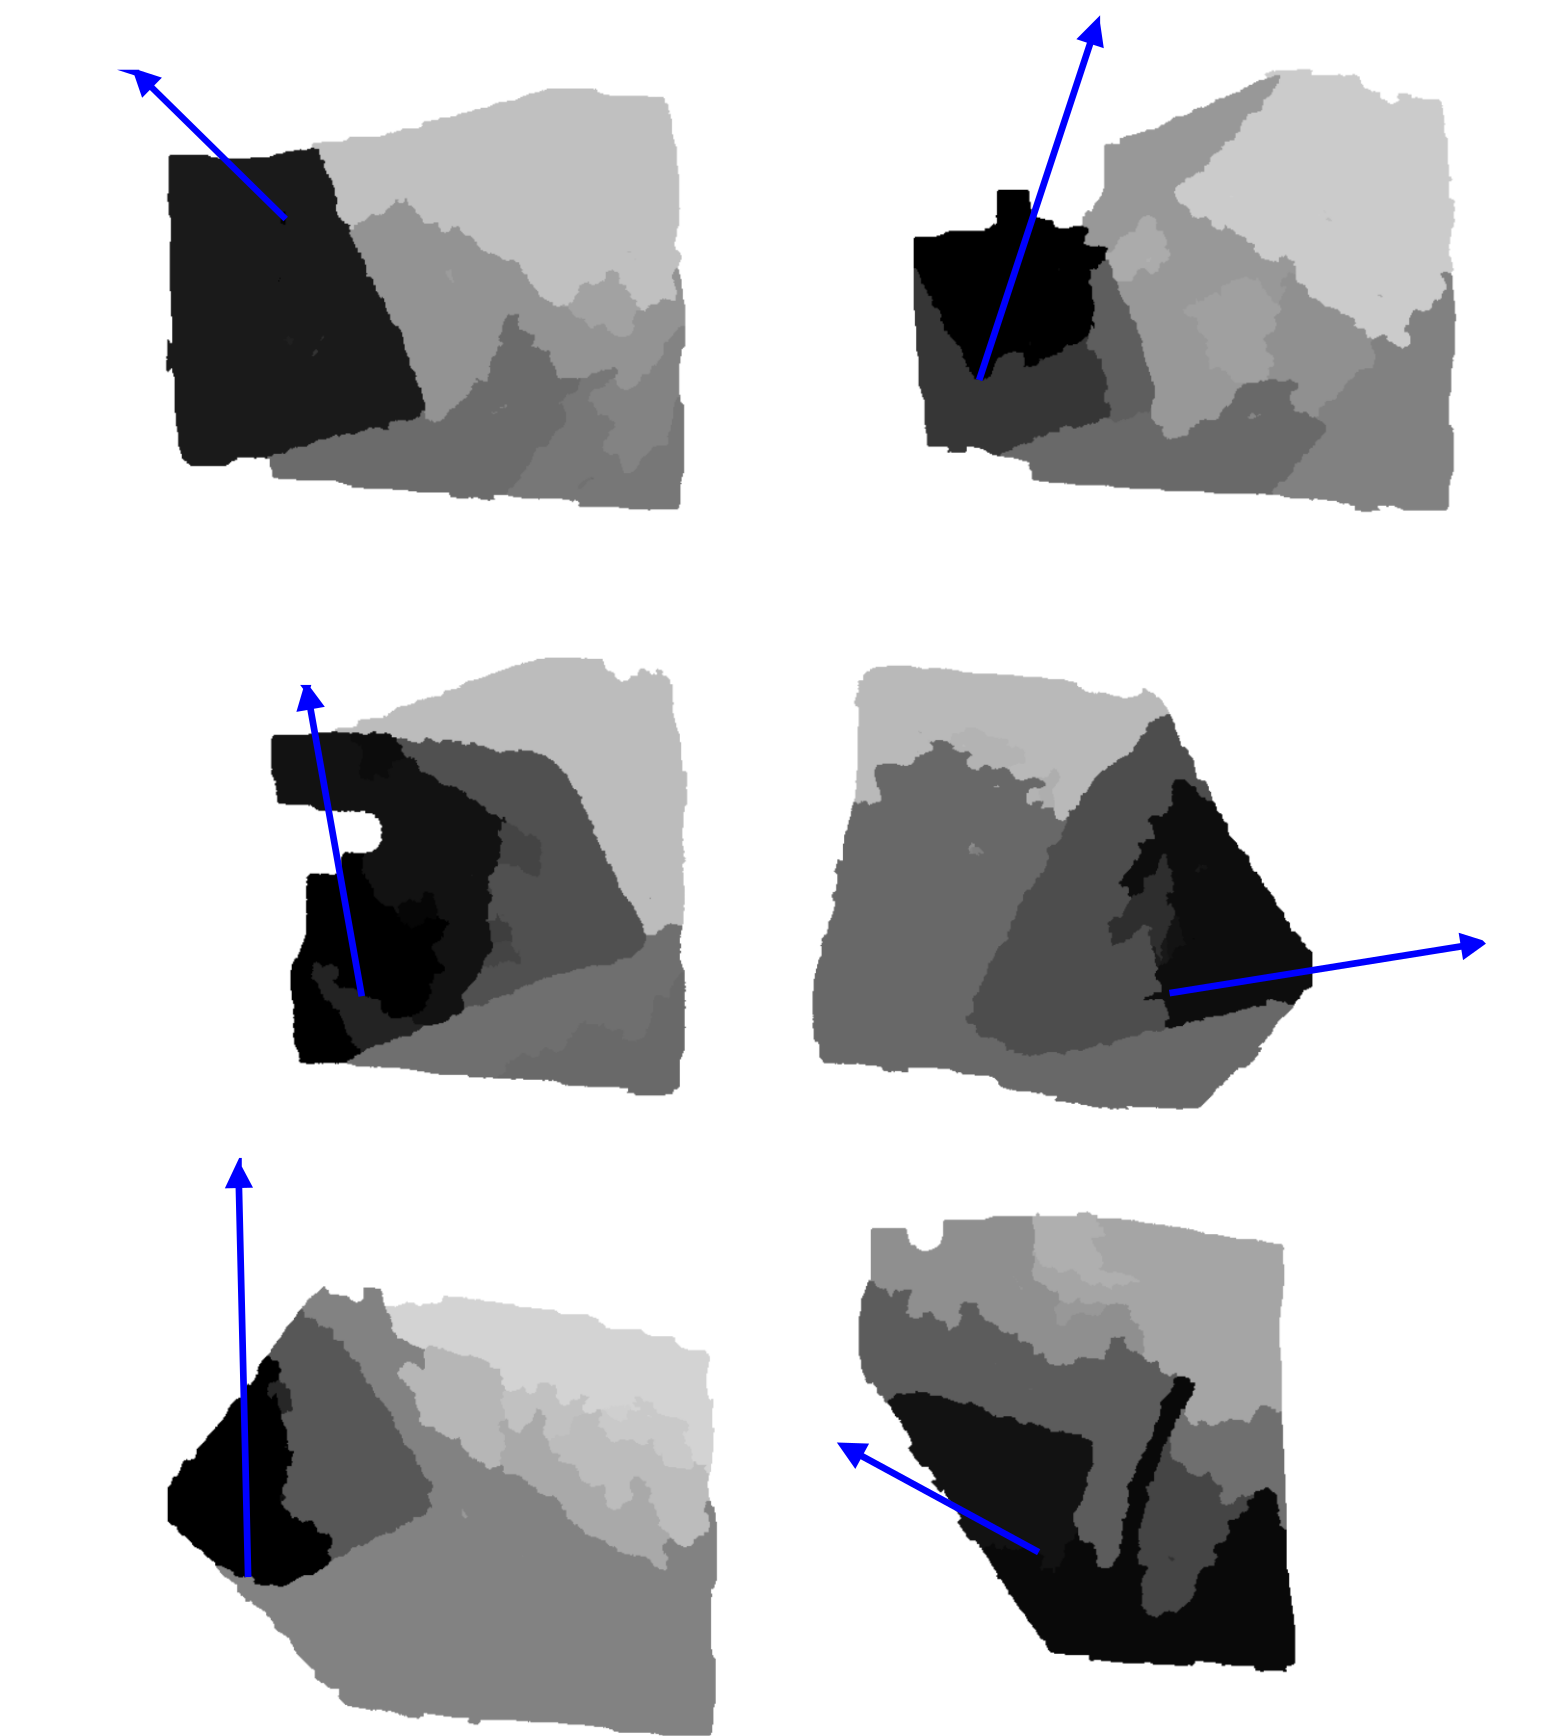
\includegraphics[width=0.45\textwidth]{figures/directions.pdf}
    \caption{Final directions calculated for each garment provided to the system. Each arrow departs where the robot should pick the fold and arrives where it should be placed.}
    \label{directions}
\end{figure}